\documentclass[a4paper,11pt]{article}

\usepackage[left= 1.5cm,text={18cm, 25cm},top=2.5cm]{geometry}
\usepackage[utf8]{inputenc}
\usepackage[T1]{fontenc}
\usepackage{times}
\usepackage{paralist}
\usepackage{graphicx}
\usepackage{textcomp}
\usepackage{enumitem}
\usepackage{amssymb}
\usepackage{amsmath}
\usepackage{xcolor}
\usepackage[ddmmyyyy]{datetime}
\usepackage{array}
\pagestyle{plain}
\pagenumbering{arabic}
\usepackage[slovak]{babel}
\usepackage{lmodern}


\renewcommand*\contentsname{Obsah}

\newdateformat{mydate}{\twodigit{\THEDAY}.{ }\shortmonthname[\THEMONTH] \THEYEAR}

\pagenumbering{arabic}

\usepackage{url}
\DeclareUrlCommand\url{\def\UrlLeft{<}\def\UrlRight{>} \urlstyle{tt}}

% \usepackage{indentfirst}

\begin{document}
\selectlanguage{slovak}

\begin{titlepage}
\begin{center}
    {\Huge \textsc{Vysoké učení technické v Brně}}
\vspace{\stretch{0.01}}
    
    {\LARGE \uppercase{FAKULTA INFORMAČNÍCH TECHNOLOGIÍ}}
    
\begin{figure}[h]
\vspace{5.0cm}
\centering

\includegraphics[scale=0.15]{logo.png}
\vspace{-10.0cm}
\end{figure}
    
\vspace{\stretch{0.382}}
	{\LARGE Projekt IMP, 2019Z}
\vspace{\stretch{0.02}}

	{\Huge \textbf{Vizuální efekty s maticovým LED displejem}}
\vspace{\stretch{0.02}}\\

{\LARGE {ARM-FITkit3}}\\
{\LARGE {Vede: M. Bidlo (bidlom@fit.vutbr.cz)}}\\

\begin{figure}[h]
\centering
{\Large {\mydate\today}}
\vspace{6cm}
\end{figure}

\end{center}
\begin{compactitem}
\item[] Vanický Jozef, xvanic09
\end{compactitem}

\end{titlepage}

\tableofcontents
\newpage

\section{Zadanie}

Cieľom projektu bola realizácia riešení aspoň dvoch netriviálnych svetelných efektov na maticovom displeji 8x8, externe pripojenom k Fitkitu3. Efekty boli ponechané na riešiteľovi, pričom aspoň pri jednom z efektov bolo za potreby využiť riadenie LED pomocou PWM.

\section{Popis ovládania a efektov}
Po pripojení fitkitu k napájaniu sa na displeji zobrazí prvý svetelný efekt. Efekty nie su nijak ovládané užívateľom a postupne sa cyklicky opakujú. V stĺpcoch budú postupne prechádzať farby červená, zelená a oranžová zhora dole. Farby sa v jednotlivých stĺpcoch každou ďalšou iteráciou menia. V jednom stĺpci sa každá z farieb vystrieda tri-krát, pričom následne nasleduje druhý svetelný efekt. Druhý svetelný efekt reprezentuje pomalé sa približovanie, kontakt, zmiešanie a nasledovné rozpínanie sa. V tomto efekte bol využitý "potenciál" RGB LED diód a pulzne šírkova modulácia, ktorú prvý efekt nemal.

\section{Popis riešenia}
Celá implementácia je v rámci súboru main.c. Projekt nie je zložitý natoľko, aby bolo potrebné rozdeliť ho do niekoľkých súborov. Zdrojový súbor je rozdelený na časť s makrami a vlastnými funkciami.


Ako prvý je inicializovaný MCU vo funckii MCUInit, ktorá vypne watchdog a inicializuje hodiny. Následne je volaná funkcia TurnClocksON() kde sa zapnú hodiny. Ako ďalšia sa volá funkcia EffectGPIO, v ktorej je volaná ďalšia funkcia PortsInitGPIO() v ktorej sú nastavené piny pre GPIO na výstup. Ide o PTA10, PTA11, PTA24, PTA25, PTA26, PTA27, PTA28 a PTA29 ktoré reprezentujú jednotlivé riadky. Následne rovnako nastavíme piny PTA6, PTA7, PTA8, PTA9 ktoré reprezentujú stĺpce 1,3,5,7 v červenej farbe, 2,4,6,8 v červenej farbe, 2,4,6,8 v zelenej farbe a stĺpce 1,3,5,7 v zelenej farbe. Následne sú defaultne všetky LED diody vypnuté.


 Ďalej sa vraciame späť do funkcie EffectGPIO() kde sa už vykonáva samotný efekt - v cykle sa na jednotlivých bitoch registru GPIO PDOR PDO zapínajú a vypínajú jednotlivé riadky a stĺpce pre dosiahnutie požadovaného efektu. Až sa cyklus vykoná 3-krát, prejdeme po spozdení funkciou delay() k inicializácii časovačov vo funkciách FTM0Init() a následne FTM1Init(), kde sa v oboch postupne vyčistí register počítadla, nastaví  sa maximálna hodnota udávajúca jas ledky do modulo registra a nastaví sa generovanie PWM na vybraných časovačoch a ich kanáloch a to konkrétne na FTM0CH3, FTM0CH4, FTM1CH0, FTM1CH1. Nakonfiguruje sa stavový a kontrolný register každého časovača.
 
 
 Následne prechádzame k vykonaniu efektu pulze šírkovou moduláciou, to prebeha volaním funkcie EffectPWM(). V tejto funkcii voláme ďalšiu a to PortsInitPWM(), kde sa rovnako ako u GPIO nastavujú všetky riadky na správny PIN. Nastavia sa na GPIO output. Tu je oproti funkcii PortsInitGPIO() rozdiel v tom že stĺpce nastavujeme na jednotlivé časovače a to na FTM0CH3, FTM0CH4, FTM1CH0 a FTM1CH1. Tiež sú tu však všetky LED diody defaultne vypnuté. Následne sa vraciame do funkcie EffectPWM() kde už sa vykonáva samotný efekt riadený PWM moduláciou a to takisto v cykle ako tomu bolo u predchodzieho efektu.

\section{Obmedzenia}
Prvá dioda na LED displeji je nefunkčná. \\Zapojenie pre PWM bolo možné realizovať maximálne pomocou 6 časovačov, čo veľmi obmedzuje v možnostiach tvorby efektov.

\newpage
\section{Schéma zapojenia}
\begin{figure}[h]
\vspace{5.0cm}
\centering
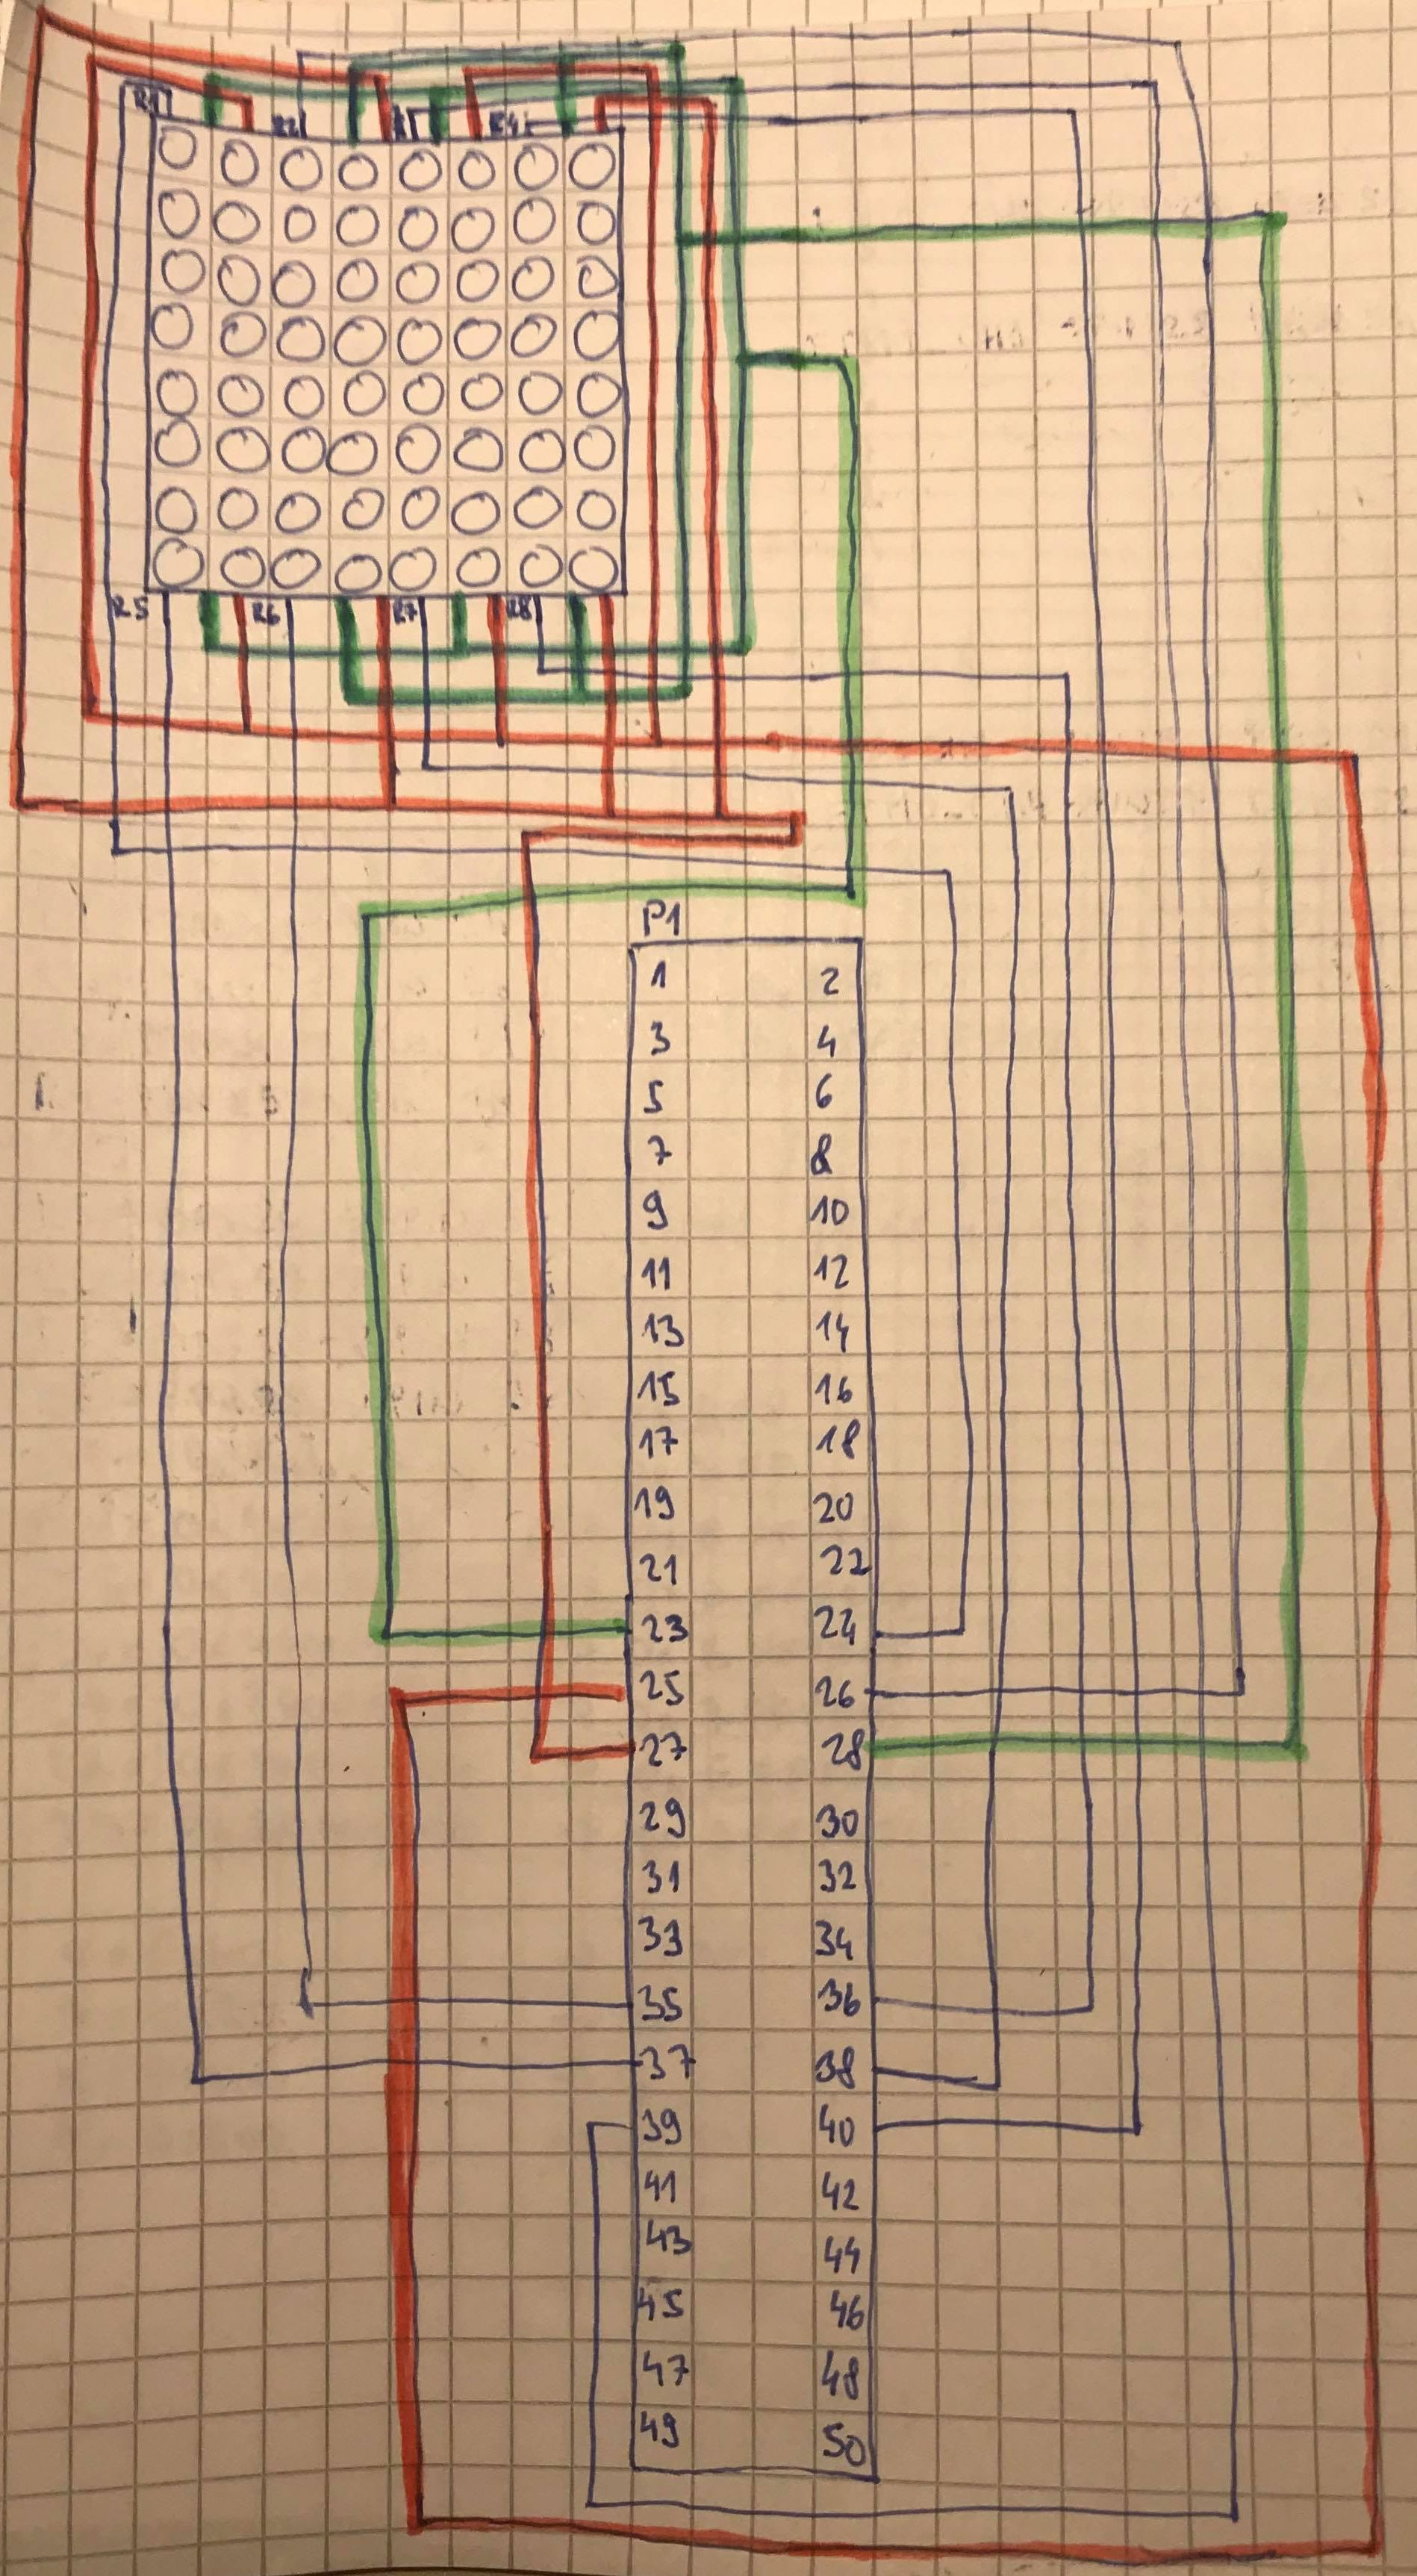
\includegraphics[scale=0.15]{foto.png}
\vspace{-10.0cm}
\end{figure}



\newpage
\newpage
\section{Zdroje}
\begin{compactitem}
\item Prezentácie predmetu IMP
\item FITkit3-demo
\item Schéma Minerva 
\item NXP K60P144M100SF2V2 
\item NXP K60 Sub-Family Reference Manual 
\end{compactitem}

\end{document}